In this chapter, we outline the method used to solve the equations governing the dynamics of the extended Prandtl-Tomlinson model, and we describe the choices of parameter ranges analyzed in the study of the same dynamics.
\section{Euler-Maruyama method}
In this part we introduce the method of numerical integration of the equations introduced in Section \ref{ourmodel}: the Euler-Maruyama method \cite{Euler}.
\\
This method is the natural extension of Euler method, a traditional method for the numerical approximation of ordinary differential equations (ODEs), to stochastic differential equations (SDEs).
\\
This approach represents one of the simplest time discrete approximations of Brownian motion, that models the random motion of particles suspended in a fluid.
\\
Ref.\cite{Euler} considers a process $X$ satisfying the following scalar stochastic differential equation
\begin{equation}
    dX(t) = a(X(t),t) dt + b(X(t),t) dW(t)
\end{equation}
on interval $0 \leq t \leq t_\text{tot}$ with initial value $X(t=0)=X_0$.
\\
Considering a discretization of $[0,t_\text{tot}]$ into $N$ equal intervals of lenght 
\begin{equation}
    dt=\frac{t_\text{tot}}{N}
    \label{eq:passo}
\end{equation}
the Euler-Maruyama approximation is a continuos time stochastic process $Y=\{Y(t) | t\in [0,t_\text{tot}]\}$ that satisfies 
\begin{equation}
    Y_{n+1} = Y_n + a(t_n,Y_n) (t_{n+1} -t_n) + b(t_n,Y_n) (W_{t_n + 1} - W_{t_n})
    \label{EulMayuEQ}
\end{equation}
where $n = 0,1,2,\dots,N-1$ and the initial value is $Y(t=0) = X_0$. Here $a$ and $b$ are the so called drift and diffusion functions evaluated at the time $t_n$.
\\
In \eqref{EulMayuEQ} there is also the following term 
\begin{equation}
    W_{t_n + 1} - W_{t_n} = \Delta W_n
\end{equation}
for $n = 0,1,2,\dots,N-1$, which represents a random Gaussian increment of the Wiener process $W(t)$.

A Wiener process $W = \{W(t)|t\geq 0\}$ is defined as a Gaussian process indexed by nonnegative real numbers $t$ with the following properties:
\begin{enumerate}
    \item $W(0)=0$ with probability equal to 1.
    \item for any time $s<t$ the increment $\Delta_{t,s} \equiv W(t)-W(s)$ follows a Gaussian distribution with mean value $\langle W(t) \rangle = 0$ and variance $Var(\Delta_{t,s}) = t-s$ .
    \item has stationary indipendent increments.
\end{enumerate}
A Wiener process is commonly called Brownian motion, but sometimes these terminologies are distinguished by their nature: the first is a mathematical process and the second a physical one.
\\
To solve equations \eqref{eq_def} the Wiener processes are Gaussian noises following the discrete-time correlation described in \cite{10.1063/5.0066008} as
\begin{equation}
    \xi(t) = \sqrt{2 k_BT \gamma dt} \hspace{0.2cm} \xi_{0}(t)
\end{equation}
is important to note that this relation is valid for discrete-time stochastic algorithms. In this relation, $dt$ represents the time step size and  $\xi_0$ denotes an uncorrelated Gaussian noise with zero mean and standard deviation $1$.
\newpage
\subsection{Time step size}
Given the number of steps and the total simulation time the time step is fixed by Eq. \eqref{eq:passo}. Since the numerical error of the integration method decreases as $dt$ is decreased, one should decrease $dt$ as much as possible. On the other hand, to accumulate significant statistics over the mechanical evolution, one often needs to run the simulation for long simulation times $t_\text{tot}$, and therefore for a large number $N$ of steps. To keep the overall computation time under control, one needs to select the integration step carefully. We now explain the method for a satisfactory determination of $dt$. As the equation is stochastic, the integration numerical error tends to hide under the stochastic noise introduced by the Wiener process. For this reason, convergence tests over $dt$ need to be carried out at $T=0$, where the Gaussian noise plays no role. This consideration leads us to a standardized numerical technique that can be outlined as follows: 
\begin{itemize}[label={\scalebox{0.4}{$\blacksquare$}}]
    \item We select an initial time step $dt$ .
    \item A relatively short $T=0$ simulation is carried out using this initial time step.
    \item The same simulation is executed using a smaller time step, typically reduced by a factor $2$.
    \item The solutions of these two simulations are compared to check for possible deviations. If these deviation are negligibly small, then the first tested time step is appropriate, and can be adopted for the actual simulations at all temperatures. Otherwise this step-reduction process is iterated until the deviations in the solution become negligibly small.
\end{itemize}
 The time step size appropriate for the adopted set of parameters $k_b$, $K$, $\gamma$, $\gamma_b$, discussed in the next section, is $dt=10^{-3}$ $U^{-1}a^2 \gamma$.
\newpage
\section{Ranges of parameters}
We discuss the choice of parameter ranges investigated in the present study.
\subsection{Temperature}
To select a suitable temperature range for the viscoelastic environment we have simulated the trajectory of the colloidal particle in condition of no-sliding and without considering the viscoelastic bath. 
This condition can be achieved by removing the coupling between the real particle and the driving stage support, namely we set the driving spring constant $K$ to $0\hspace{0.1cm}Ua^{-2}$
\begin{figure}
    \centering
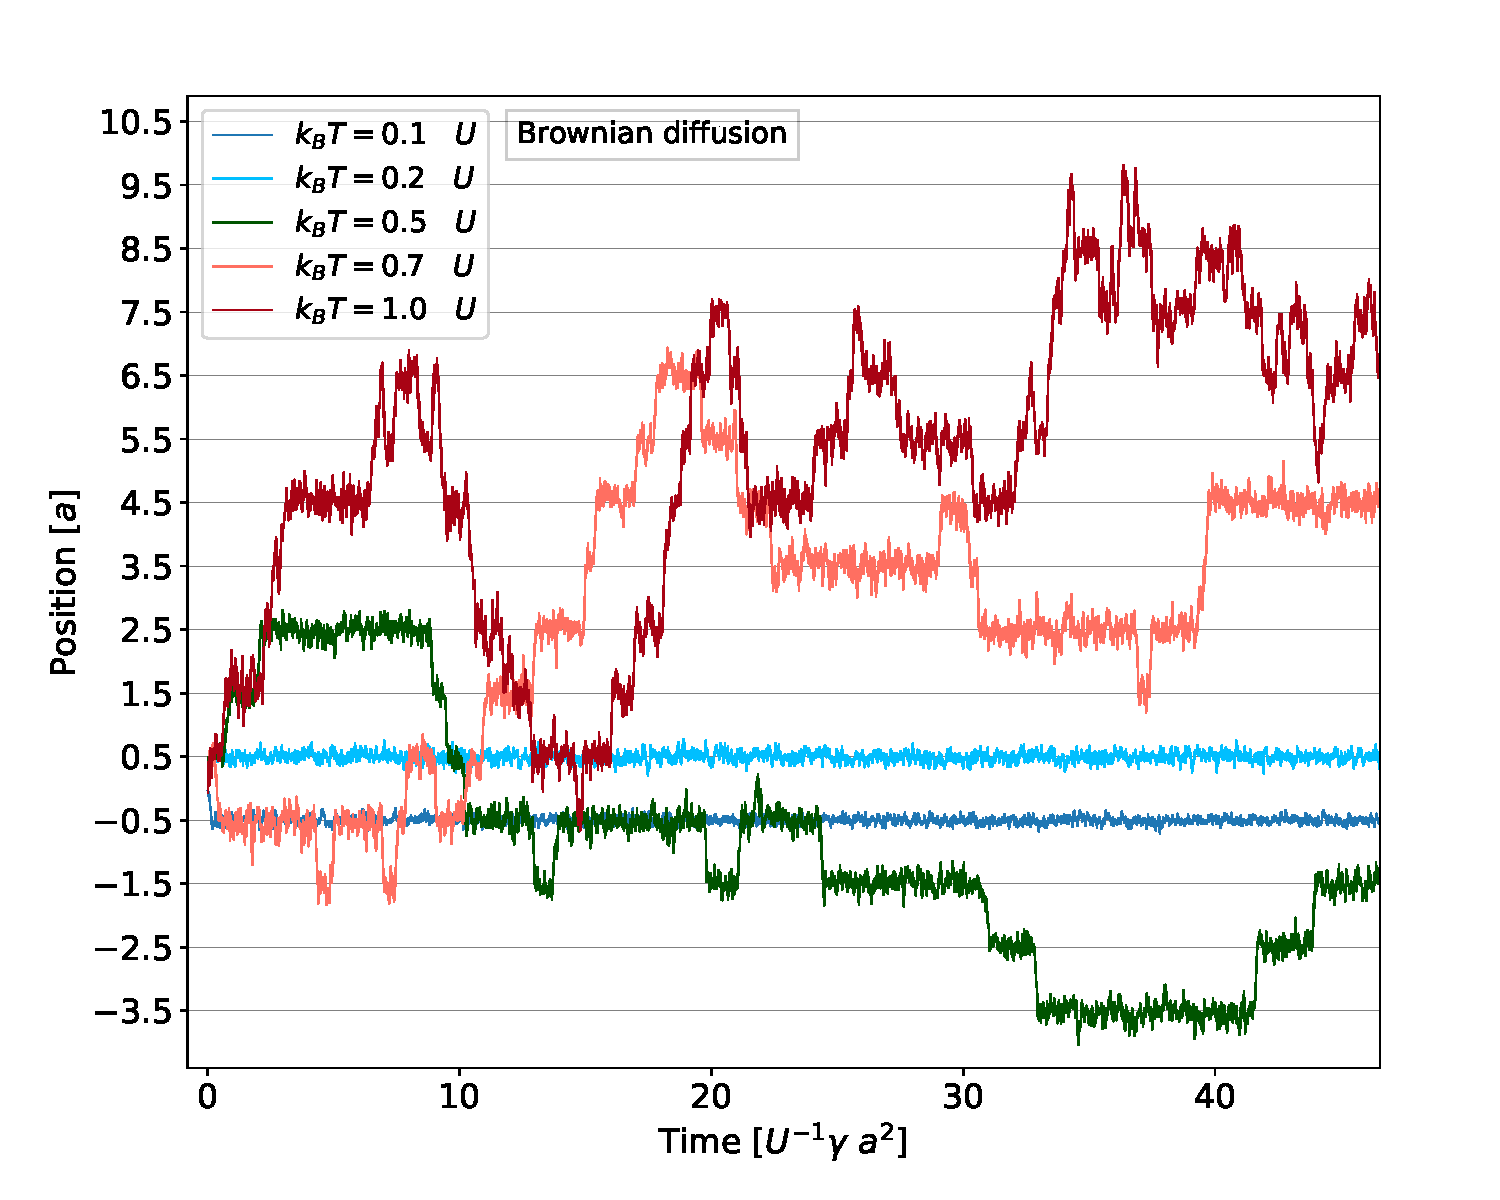
\includegraphics[width=0.9\textwidth]{scelta_temperatura.pdf}
\caption{Examples of solutions of the equation of motion \eqref{eq_def} started at $x(0)=0$, in no-driving conditions ($K=0\hspace{0.1cm}Ua^{-2}$) for a standard Brownian system ($k_b=0\hspace{0.1cm}Ua^{-2}$), at the few indicated values of temperature $T$ (standard thermal diffusion). The thin horizontal lines indicate the positions of the potential minima.}
\label{graph_Tchoice}
\end{figure}

Figure \ref{graph_Tchoice} reports the outcome of a few simulations of pure diffusion for a few different temperatures.
This figure illustrates how the particle moves under the competing effects of thermal fluctuations and of the sinusoidal corrugation potential.
\begin{itemize}[label={\scalebox{0.4}{$\blacksquare$}}]
    \item When $k_BT=0.1/0.2 \hspace{0.1cm}U$ the particle drops in one of the adjacent minima, then oscillates around the minimum position. Inter-minima thermally activated jumps are extremely rare.
    \item When $k_BT=0.5\hspace{0.1cm}U$ the random forces leave the particle at a minimum for the most of the simulation time, but are sufficiently strong to promote occasional jumps, and therefore a visible diffusive motion.
    \item When $k_BT=0.7 / 1\hspace{0.1cm}U$ minima and intermediate barriers are both significantly explored, the inter-minima jumps are so frequent that diffusive events dominate.
\end{itemize}
The time evolution for the non-Markovian model is qualitatively similar, but with less frequent inter-well jumps (see Fig.\;\ref{fig:T_kb15}).
\begin{figure}
    \centering
    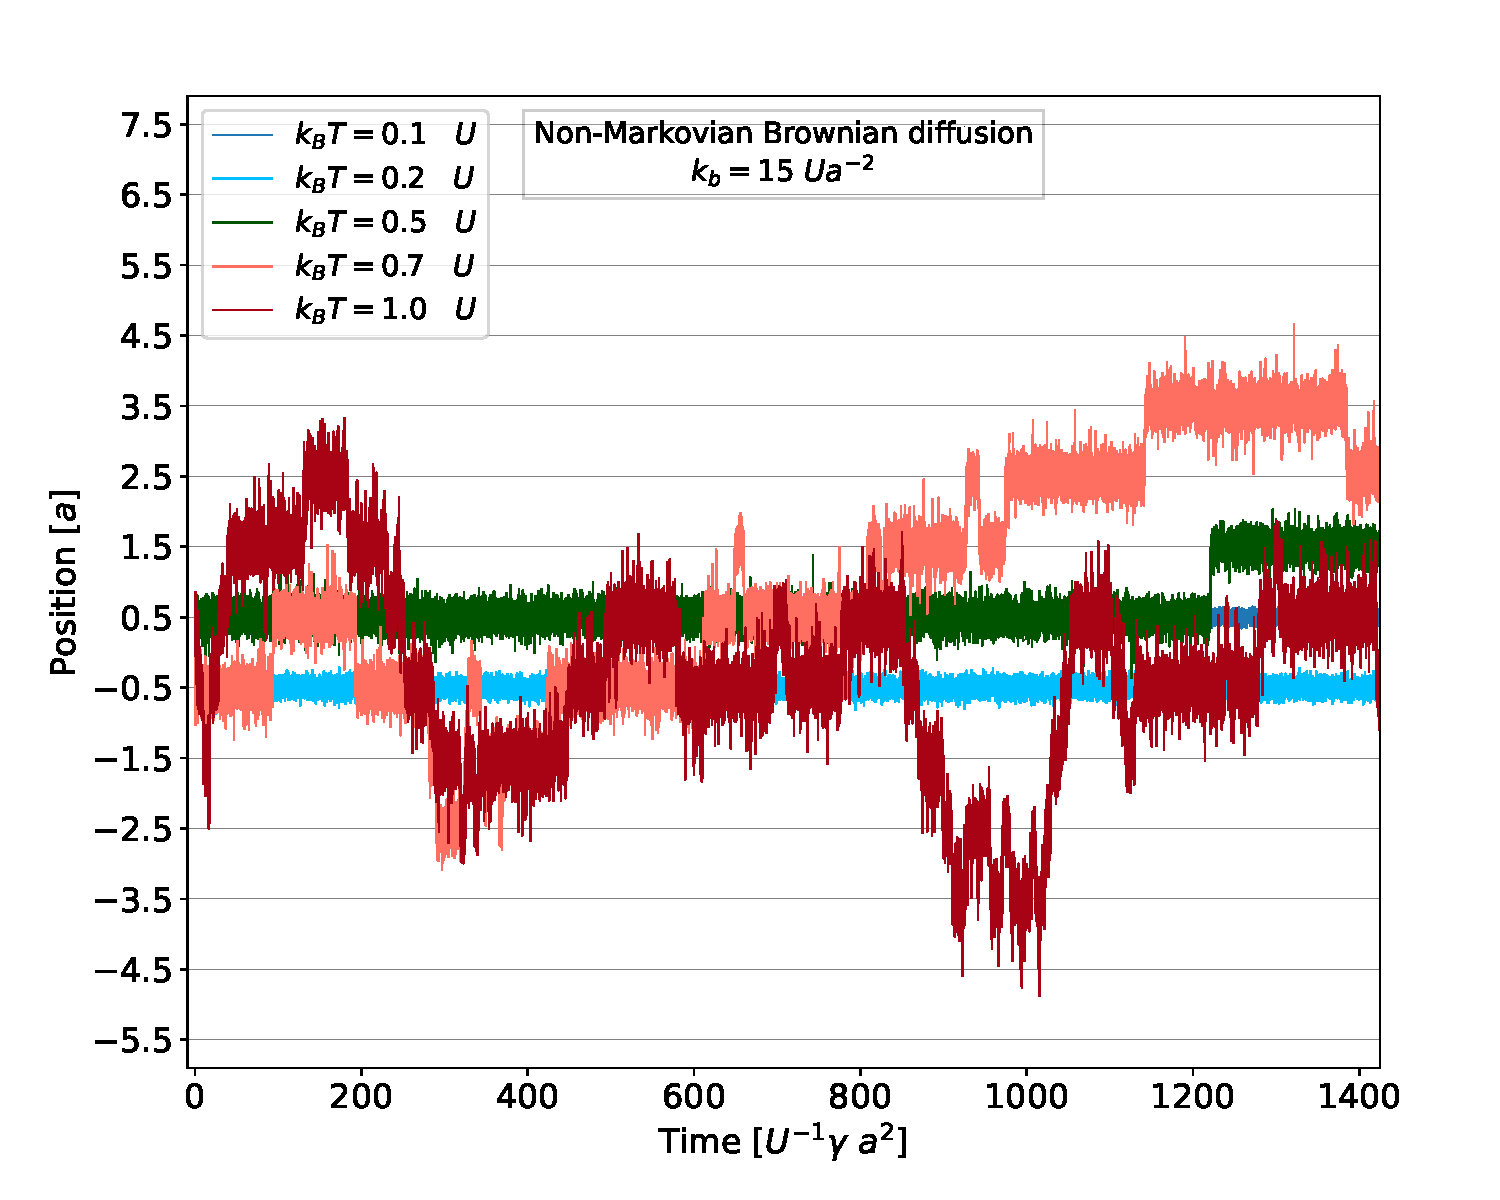
\includegraphics[width=0.9\textwidth]{scelta_temperatura_kb15.pdf}
    \caption{Same as Fig.\,\ref{graph_Tchoice}, but for a Brownian particle in a non-Markovian  environment with $k_b=15\; Ua^{-2}$}
    \label{fig:T_kb15}
\end{figure}
Since we are interested in studying the statistics of barrier jumps, we see that a suitable temperature is $k_BT = 0.5\hspace{0.1cm}U$, which is large enough that jumps occur at a fair rate, but not so large that the residence time at the potential wells becomes negligible.
\subsection{Damping coefficients and spring constants}
In this part, we refer to the experiments described in Ref.\cite{ginot2022} to tune the parameters used in our simulations. Specifically, Ref.\cite{ginot2022} employs damping coefficients $\gamma =\SI{0.186}{\micro\newton\second\meter^{-1}}$ and $\gamma_b = \SI{1.44}{\micro\newton\second\meter^{-1}}$. To adopt a similar ratio of viscous coefficients in our model, we consider  $\gamma_b = 7 \gamma$. With regard to the spring constant $k_b$, linking the true particle to the non-Markovian environment fake particle, to fix its value we identify the elastic energy accumulated in that spring when the true and fake particles sit at the bottom of adjacent wells. In the experiment of Ref.\cite{ginot2022}, a spring constant $k_b=\SI{0.4}{\micro\newton\meter^{-1}}$ is used. The distance between two minima is $2x_m =\SI{0.64}{\micro\meter}$ therefore the elastic energy is given by 
\begin{center}
    $U_{k_b} = \dfrac{1}{2}k_b (2 x_m)^2 \simeq 8.19 \cdot 10^{-20} \;\SI{}{J}$
\end{center}
The potential barrier in the model of Ref.\cite{ginot2022} 
\begin{center}
    $\Delta U = 2.1\hspace{0.1cm} k_BT \simeq 8.65 \cdot 10^{-21}\;\SI{}{\joule}$
\end{center}
because the experiments are conducted at $T=\SI{25}{\degreeCelsius}=\SI{298.15}{\kelvin}$. As a result 
\begin{center}
    $\dfrac{1}{2}\dfrac{k_b (2 x_m)^2}{\Delta U} \simeq 9.47$
\end{center}
To obtain a similar ratio in our model where the height of the potential barrier is twice of the natural units $\Delta U = U_0 = 2\hspace{0.05cm}U$. In our model, two consecutive minima are separated by a distance $a$; therefore, we can express the elastic energy as
\begin{center}
    $U_{k_b}  = \dfrac{1}{2}k_b a^2$
\end{center}
By comparing the quantities just described, we observe that the corresponding value of harmonic spring $k_b$ in our units would equal $37.9 \hspace{0.1cm} Ua^{-2}$, thus we explored comparable although slightly smaller values $k_b= 15 \hspace{0.1cm} Ua^{-2}$ and $k_b= 20 \hspace{0.1cm} Ua^{-2}$.

As for the elastic spring constant $K$, it describes how strongly the colloidal particle is coupled to the sliding stage. 
A very small value of $K$ implies that it may take several thousands of time units for the colloidal particle to start following the slider, thus a steady state may be hard to reach. On the other hand, with a large $K$ the particle would move close to the driving stage and thus may not exhibit significant effects of the interaction with the corrugation potential and the non-Markovian bath particle, as discussed for standard PT model in Section \ref{PTmodel}, and specifically around Eq.\eqref{eta}. As a fair compromise, for all driven simulations we adopt $K=0.001\hspace{0.1cm}Ua^{-2}$.
\subsection{Velocity}
The choice of the slider velocity $v$ range to investigate is based on the fact that it determines the particle's average waiting time $t_\text{w} = a/v$ in the potential minima. For the effects of the non-Markovian environment to be significant, we need $t_\text{w}$ to be comparable to or longer than the typical times between thermally-activated interwell jumps. As shown in Figure \ref{graph_Tchoice}, thermal jumps can occur every few times $t_0$ for $k_BT=0.5\hspace{0.1cm}U$. As a result, interesting physics is expected for 
\begin{center}
    $v \lesssim \dfrac{a}{10\hspace{0.1cm}t_0} = 0.1 \hspace{0.1cm} U a^{-1}\gamma^{-1}.$
\end{center}
On the other hand, a very low velocity would cause the slider to advance by only a few units of length $a$ even in very long simulations. For instance, at a velocity of $10^{-6}\; Ua^{-1}\gamma^{-1}$, the stage would move by one unit of length $a$ in a simulation with $t_\text{tot}=10^6\hspace{0.1cm}t_0$ that requires one billion time steps.
Extremely low velocities $v < 10^{-4} Ua^{-1}\gamma^{-1}$ although potentially useful to investigate the velocity-dependence of the friction force in the PT model and in its extension are too challenging for this preliminary study, and we will not attempt them.